\documentclass[ignorenonframetext]{beamer}
\usepackage{beamerthemesplit}
\usepackage{amssymb}

%\documentclass[a4paper]{article}
\usepackage{beamerarticle}
\usepackage{verbatim}

\usepackage{../fhnw-beamer}

%\mode<article>{\usepackage{fullpage}}
%\mode<presentation>{\usetheme{Berlin}}

\date{\today}
\author{rolf.schmutz@fhnw.ch}
\institute{FHNW}
\title {Netzwerke und Datenkommunikation\\B-LS-MI 004\\Physical Layer}


\begin{document} % ===============================================================

\section{NDK B-LS-MI 004: L2}



\begin{frame}
\titlepage
\end{frame}

\begin{frame}
\frametitle{Ziele}
\begin{itemize}
	\item{Repr\"asentation des Quellsignals auf elektromagnetischer Ebene}
	\item{Codierung des Quellsignals (Abgek\"urzt)}
	\item{Verfahren zur Leitungscodierung der Daten aus einem Quellenstrom}
	\item{Techniken in Bezug auf Basisband- und Breitband-Kommunikation (Modulation)}
	\item{Fehlererkennung und -Korrektur}
\end{itemize}
\end{frame}





\begin{frame}
\frametitle{Einfachste Bit-Serielle Daten\"ubertragung}
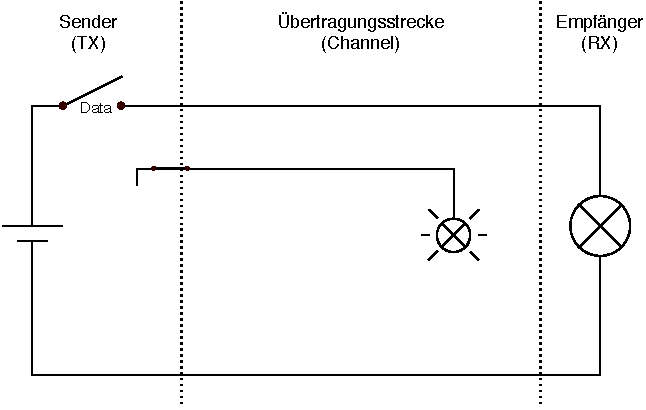
\includegraphics{simplest-serial}

\begin{itemize}
  \item ``Hello World!'' soll \"ubertragen werden
\end{itemize}
\end{frame}
%% Linu/URL/referenz: \myurl{http://www.rfc-editor.org/rfc/pdfrfc/rfc1918.txt.pdf}

Will this be rendered in Article Mode?

\begin{frame}
\frametitle{Probleme}
\begin{itemize}
  \item wie wird ``Hello World!'' als Abfolge von Licht/kein-Licht (0, 1) dargestellt? (Quellcodierung)
  \item wann beginnt die Nachricht (oder einzelne Buchstaben), wann endet sie?
  \item wie k\"onnen einzelne gleiche ``bits'' getrennt werden? z.B. ``o''=01101111
\end{itemize}
\end{frame}


\begin{frame}
\frametitle{Quellencodierung (source-coding) 1/2}
\begin{block}{}
  Das ist die Repr\"asentierung von Informationen in bin\"arer (numerischer) Form, 
  also nicht Programm-Quellcode/sourcecode
\end{block}

\begin{itemize}
  \item es wird eine \"Ubereinkunft/Tabelle ben\"otigt, die die Information in numerischer Form (Bitmuster) festlegt (code-point)
  \item es gibt eine Vielzahl von Codierungen f\"ur verschiedene Datenformate
\end{itemize}
  \begin{block}{}{Die Codierung muss auf beiden Seiten bekannt sein und ist nicht gleich ``Verschl\"usselung''}\end{block}
\end{frame}


\begin{frame}
\frametitle{Quellencodierung (source-coding) 2/2}

F\"ur unsere Zwecke benutzen wir die alterw\"urdige ASCII-Codierungstabelle (ohne Kontrollzeichen):

\begin{table}[htdp]

  \begin{center}
    \begin{tabular}{|l|l|}
      \begin{tiny}\verbatiminput{asciitable.txt}\end{tiny} | z.B. ``H'' = 48_{16} = 0100'1000_{2} \\
    \end{tabular}
  \end{center}
\end{table}

\end{frame}

\end{document}